\section{Sprint 2}

\subsection{Goals for the sprint}
In the second sprint the team focused on providing the customer with a working prototype to further develop the requirements specification. Furthermore, a working prototype might help the customer see how the team envisioned the app and its functions. Lastly, work on the server application began to form the foundation a framework of functions that the android app could use.

\subsection{Design}
Before implementing the specification that was approved by the customer, the team built prototypes of the design in sketching programs to ensure a consistent and clean design throughout the app. 

\subsection{Development}
As the GUI design neared an end, the team started implementing the features the customer specifically asked to have included in the first iteration of the app.

\subsubsection{Server}
The groundwork for the apps server was put down in sprint 2. Using Dropwizard the development team started the implementation of the functions available to the app.

\subsection{Results}

\subsubsection{Improper use of Scrum tool}
As mentioned in section~\ref{sec:scrumtools}, the team used a lot of time on deciding on which Scrum tool to use for the project management. Although our choice fell on Yodiz, the team was in lack of any previous experience with the tool, and despite the team's efforts to get acquainted with the tool, a misunderstanding arose and was not discovered until the end of the second sprint.

The misunderstanding, displayed in figure~\ref{fig:wrongUse}, was that the team assumed one could add multiple individuals as responsible on a particular task, while Yodiz' functionality only assigned the time spent to the individual that either created the task or was assigned as owner of the task.

As a result, it appeared as if only singular individuals performed the tasks, even though the entire team in reality was participating, which was also reflected in the burndown charts and the generated gantt diagram. 

To sort out this issue, the team went through old meeting reports and timesheets to figure out which members of the team that had actually participated on the particular task, and added new tasks and the time spent to the members that at the time had not recorded this information, as shown in figure~\ref{fig:addsTasks}.

This issue was unfortunate, but not insurmountable, and also not a critical issue for the overall progress of the project.

\begin{figure}[H]
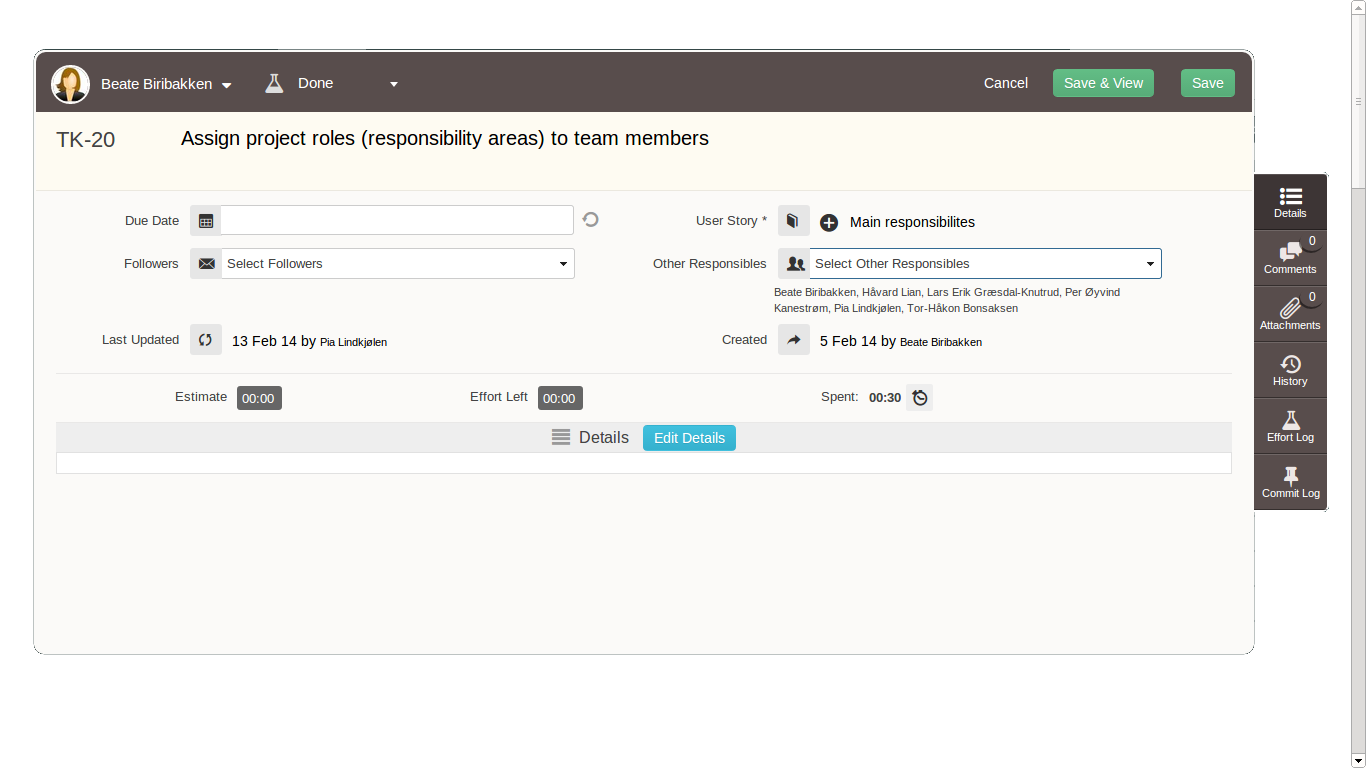
\includegraphics[width=\textwidth]{ch/sprints/fig/wrongUse.png}
\label{fig:wrongUse}
\end{figure}

\begin{figure}[H]
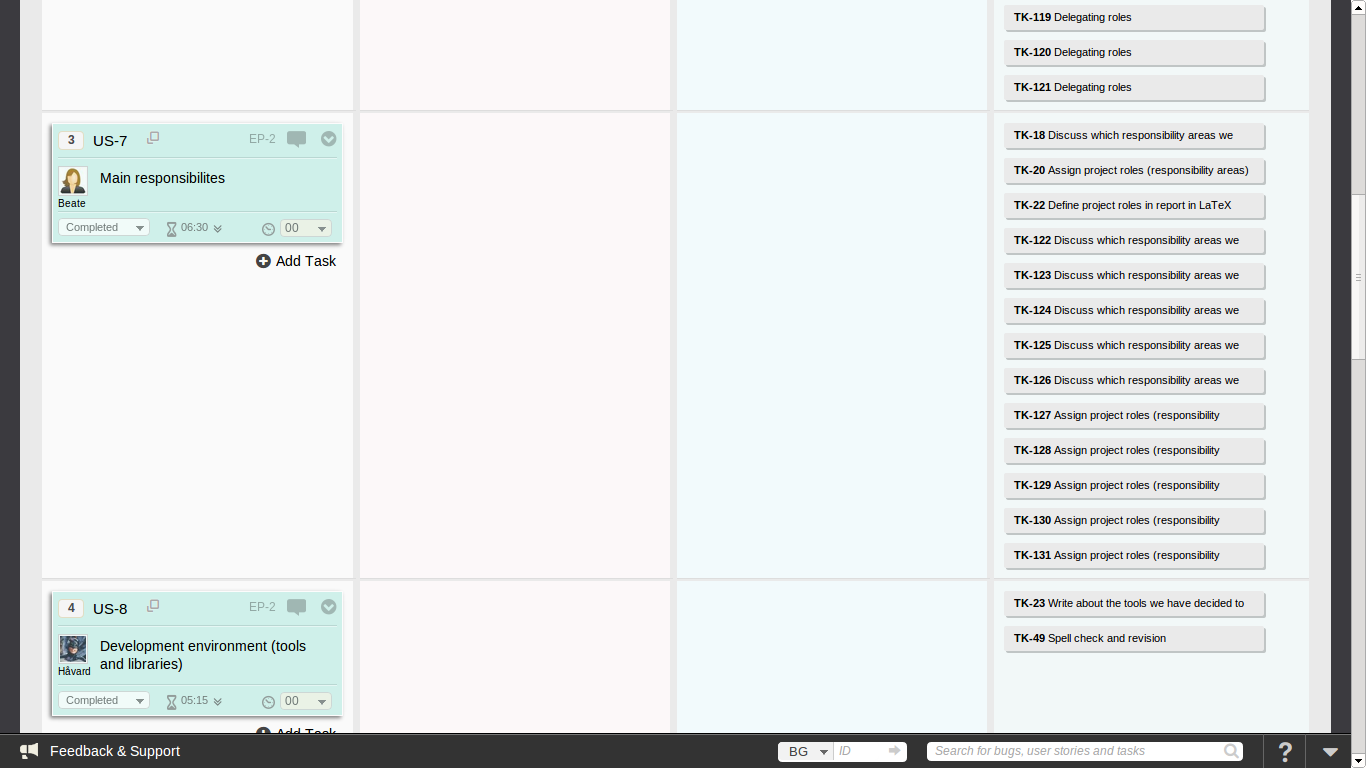
\includegraphics[width=\textwidth]{ch/sprints/fig/addsTasks.png}
\label{fig:addsTasks}
\end{figure}

\subsubsection{\todo[inline]{Working away from the team}}
One of the team members, Lars Erik, had to make a sudden trip abroad due to death in the family. He stayed away from the team for a total for 12 days. Prior to departure the team divided the tasks with a lighter workload assigned to Lars Erik, as described in the risk analysis. Even with the redistributed workload the team and Lars Erik in particular found the distance and time difference to be a bigger problem than expected. Some work was left undone and had to be picked up at the end of the sprint or pushed to the next sprint. The team learned that the impact of such leaves of absence should probably be overestimated rather than underestimated in the eventuality of another event.

\subsubsection{General results from sprint 2}
The customer was happy with progress on the prototype, and provided rich and detailed feedback on how the app should be improved for the next iteration. The sprint was deemed successful by the team members.